\title{Chapter 4, Section 2. Exercises 1, 2, and 4 through 9}
\author{
	MTH 594, Prof. Mikael Vejdemo-Johansson \\
	Differential Geometry Independent Study \\
	\\
	Matthew Connelly \\
}
\date{\today}



\documentclass[12pt]{article}

\usepackage[top=.5in, bottom=.75in, left=1in, right=1in]{geometry}
\usepackage{amssymb}
\usepackage{amsmath}
\usepackage{graphicx}
\usepackage{subcaption}
\usepackage{pgfplots}
\usepgfplotslibrary{colormaps,fillbetween}
\pgfplotsset{compat=1.10}

\newcommand{\ulind}[1]
{
\noindent
\underline{#1}\\\\
\indent
}


\begin{document}
\maketitle

\section*{Exercise 4.2.4}
Show that the ellipsoid
$$
\frac{x^2}{p^2} + \frac{y^2}{q^2} + \frac{z^2}{r^2} = 1,
$$

where $p$, $q$ and $r$ are non-zero constants, is a smooth surface.

\vspace{1cm}
\hrule
\vspace{1cm}
\noindent

Let $S$ equal our ellipsoid; $S$ can be parametrized as the following rotational solid:
$$
\sigma = (p \ \cos u \ \cos t, q \cos u \ \sin t, r \sin u)
$$

\begin{figure}[h!]
	\centering
	\begin{subfigure}[b]{0.5\linewidth}
		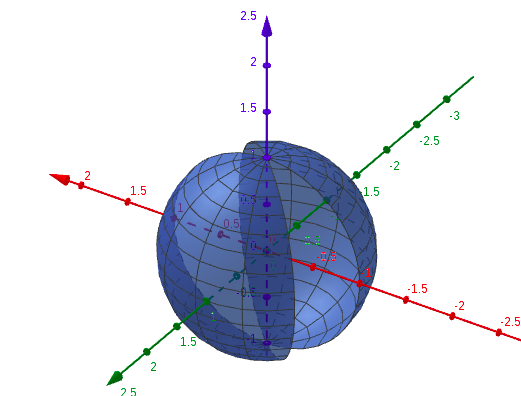
\includegraphics[width=\linewidth]{./assets/4-2-4/sphere-rotational.png}
	\end{subfigure}
\end{figure}
\indent

\clearpage

\ulind{Demonstrating smoothness via partial differentiation}
If $\sigma$ is smooth, then $\sigma \in C^n$; it is differentiable continuously to order $n$. The first partial derivatives are:

$$
\sigma_t = (-p \cos u \ \sin t, q \cos u \ \cos t, 0)
$$
$$
\sigma_u = (-p \cos t \ \sin u, -q \sin t \ \sin u, r \cos u)
$$

Since $\sin $ and $\cos \in C^\infty$, it is then implied that $\sigma \in C^\infty$, making $\sigma$ smooth.\\

\ulind{Showing that $\sigma$ is a surface via its atlas}
To be a surface, $\sigma$ must have an atlas.\\

Let the atlas of $\sigma$ consist of the patches $\sigma_U$ and $\sigma_{\widetilde U}$, which map $U$ and $\widetilde U$ to $S$:\\

$$
\sigma_{U} : U \rightarrow S
$$
$$
\sigma_{\widetilde U} : \widetilde U \rightarrow S
$$

where $U$ and $\widetilde U$ are defined as follows:

$$
U = \lbrace t, u \ | \ 0 < t < 2 \pi, -\frac{\pi}{2} < u < \frac{\pi}{2} \rbrace
$$

$$
\widetilde U = \lbrace t, u \ | \ 0 < t < \pi, 0 < u < 2 \pi \rbrace
$$

\begin{figure}[h!]
	\centering
	\begin{subfigure}[b]{0.4\linewidth}
		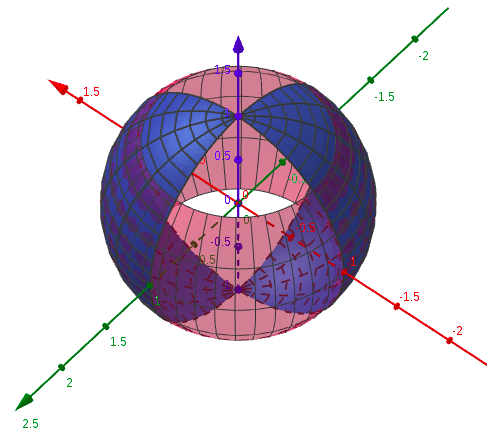
\includegraphics[width=\linewidth]{./assets/4-2-4/sphere-atlas.png}
	\end{subfigure}
\end{figure}
\indent

Pictured above is this atlas of $S$. As $\sigma_u$ (in red) closes about the north and south poles of $S$ (not visible), $\sigma_{\tilde{u}}$ (in blue) closes like a shell.
\end{document}
